 %%%%%%%%%%%%%%%%%%%%%%%%%%%%%%%%%%%%%%%%%%%%%%%%%%%%%%%
% Please note that whilst this template provides a
% preview of the typeset manuscript for submission, it
% will not necessarily be the final publication layout.
%
% letterpaper/a4paper: US/UK paper size toggle
% num-refs/alpha-refs: numeric/author-year citation and bibliography toggle

%\documentclass[letterpaper]{oup-contemporary}
\documentclass[a4paper,num-refs]{oup-contemporary}

%%% Journal toggle; only specific options recognised.
%%% (Only "gigascience" and "general" are implemented now. Support for other journals is planned.)
\journal{gigascience}

\usepackage{graphicx}
\usepackage{siunitx}

%%% Flushend: You can add this package to automatically balance the final page, but if things go awry (e.g. section contents appearing out-of-order or entire blocks or paragraphs are coloured), remove it!
% \usepackage{flushend}

\title{NanoGalaxy: A Galaxy tool kit and workflows for nanopore and Illumina NGS de novo sequence assembly}

%%% Use the \authfn to add symbols for additional footnotes, if any. 1 is reserved for correspondence emails; then continuing with 2 etc for contributions.
\author[1,\authfn{1}]{Willem~de~Koning}
\author[1]{Saskia~Hiltemann}

\affil[1]{Erasmus Medical Center, Department of Pathology, Wytemaweg 80, 3015 CN, Rotterdam, The Netherlands}
\affil[2]{Bioinformatics Group, Department of Computer Science, University of Freiburg, 79110 Freiburg im Breisgau, Germany}

%%% Author Notes
\authnote{\authfn{1}w.dekoning.1@erasmusmc.nl}

%%% Paper category
\papercat{Technical Note}

%%% "Short" author for running page header
\runningauthor{de Koning et al.}

%%% Should only be set by an editor
\jvolume{00}
\jnumber{0}
\jyear{2017}

\begin{document}

\begin{frontmatter}
\maketitle
\begin{abstract}
%%The Abstract (250 words maximum) should be structured to include the following details: \textbf{Background}, the context and purpose of the study; \textbf{Results}, the main findings; \textbf{Conclusions}, brief summary and potential implications. Please minimize the use of abbreviations and do not cite references in the abstract.

\textbf{Background:} NanoGalaxy is a nanopore sequence analysis Galaxy tool kit for de novo assembly of metagenomic genomes and plasmids, including “end to end” workflows and web reporting for antimicrobial resistance (AMR) detection from clinical material.

\textbf{Results:} The user-friendly workflows enable the clinical researcher to analyse whole shotgun metagenomic data from both nanopore and Illumina next generation sequencing (NGS) to give superior detection of pathogen resistance from both the genomic and plasmid level.  We demonstrate the utility of NanoGalaxy to determine the pathogenicity from clinical NGS data.

\textbf{Conclusions:} NanoGalaxy contains tools that cover quality control, de novo assembly, species and assembly detection, AMR detection and reporting of the analysis. The tools are made available in the Galaxy Tool Shed, and is accompanied by a Galaxy training manual (\url{https://training.galaxyproject.org}). The goal is to create a user-friendly environment where researchers can choose their nanopore analysis tools or pipelines based on their research question, making their research reproducible. 
\end{abstract}

\begin{keywords}
Metagenomics; Galaxy; Reproducibility; Antibiotic resistance; Workflow; Plasmid
\end{keywords}
\end{frontmatter}

\section{Findings}
\subsection{Background}
According to the World Health Organization (WHO) and the Organisation for Economic Co-operation and Development (OECD), AMR has become one of the biggest threats to global health, food security and development \cite{OrganisationforEconomicCo-operationandDevelopment2017, WorldHealthOrganization2018}. The misuse of antibiotics in medical, veterinary and agricultural sectors contributes to the rise of antibiotic resistant pathogens. An increase in AMR may ultimately lead to an era where common infections could be lethal again. It is suspected that around 50.000 lives per year are lost due to AMR infections within the USA and Europe \cite{Simlai2016}. AMR infections are expected to increase, reaching 10 million deaths per year by 2050 \cite{ONeil2014}. To prevent this, AMR detection in samples (from all organisms) needs to be faster and be done at the subject's site.

Detection of resistant bacteria provides vital information for infection control measures. Therefore, determination of AMR is important and progressing with new innovations. The conventional methods for identification involve culturing and can take a few days or weeks to complete \cite{Quick2015}. Moreover, not all species are susceptible to laboratory-based culturing \cite{Mitsuhashi2017}. Therefore, DNA-sequencing technology is used to reduce the sample-to-result time. Illumina sequencing is the most common sequencing method, but has difficulties identifying repetitive insertion sequences usually found flanking the horizontally acquired genes often associated with AMR \cite{Ashton2014}. Furthermore, the structure of the DNA cannot be determined with short-read sequencing. Thus, the use of nanopore sequences is proposed. The disadvantage of nanopore is the high error rate, but by combining short- and long-read sequencing methods, the strengths of both techniques can help overcome these problems.

Due to the large amount of data created by nanopore and Illumina NGS sequencing, assembly is a complex, difficult to reproduce and computationally intensive analysis. Hence, NGS sequence data must be processed by refined work-flows which can requisite bioinformatics skills \cite{Hemlata2016}. Each step of the analysis may require a set of different tools or software. For example de novo assembly is done through alignment, assembly and polishing tools which all require multiple parameters. Minimap2 designed for pairwise alignment, cannot be used as standalone for de novo assembly, therefore miniasm and racon are also used. This makes it more complex as they are command-line tools, which require extensive computational resources. 

The Galaxy platform implements a user-friendly interface to accommodate command-line tools with their dependencies and refined work-flows needed for assembly of NGS data. This empowers researchers to do powerful analysis without the need for programming experience. Galaxy offers a wide range of tools for over 125 subjects. It has over 7000 citations, and with more than 7200 tools it is widely used in the biological science community \cite{Galaxycitations, Galaxytoolshed}. NanoGalaxy integrates the NGS assembly tools for a user-friendly, but powerful platform for ultimately on-site analysis of antimicrobial resistance.


\subsection{Results}

\subsubsection{Tool kit and workflows}
The incorporation of the nanopore tools in the Galaxy platform result in the tool kit, NanoGalaxy, containing diverse
applications for the analyses of nanopore sequences (Table \ref{tab:NanoGalaxyToolkit}).

\begin{table}[b!]
\caption{NanoGalaxy tool kit.}\label{tab:NanoGalaxyToolkit}
\begin{tabularx}{\linewidth}{l l l}
\toprule
Category & Tool name & Github repository\\
\midrule
De novo genome assembly         &            &                                               \\
                                & Flye       & \url{https://github.com/fenderglass/Flye}     \\
                                & Canu       & \url{https://github.com/marbl/canu/}          \\
                                & Unicycler  & \url{https://github.com/rrwick/Unicycler}     \\
                                & Wtdbg2     & \url{https://github.com/ruanjue/wtdbg2}       \\
                                & Miniasm    & \url{https://github.com/lh3/miniasm}          \\
                                & Racon      & \url{https://github.com/isovic/racon}         \\
                                & Spades     & \url{https://github.com/ablab/spades}         \\
Long-read mapping               &            &                                               \\
                                & Minimap2   & \url{https://github.com/lh3/minimap2}         \\
                                & GraphMap   & \url{https://github.com/isovic/graphmap}      \\
Polishing, QC and preprocessing &            &                                               \\
                                & Nanopolish & \url{https://github.com/jts/nanopolish}       \\
                                & Porechop   & \url{https://github.com/rrwick/Porechop}      \\
                                & Filtlong   & \url{https://github.com/rrwick/Filtlong}      \\
                                & Poretools  & \url{https://github.com/arq5x/poretools}      \\
                                & Pilon      & \url{https://github.com/broadinstitute/pilon} \\
Visualization                   &            &                                               \\
                                & Nanoplot   & \url{https://github.com/wdecoster/NanoPlot}   \\
                                & Bandage    & \url{https://github.com/rrwick/Bandage}       \\
Taxonomy and metagenomics       &            &                                               \\
                                & Kraken2    & \url{https://github.com/DerrickWood/kraken2}  \\
                                & PlasFlow   & \url{https://github.com/smaegol/PlasFlow}     \\
                                & Staramr    & \url{https://github.com/phac-nml/staramr}     \\
Methylation                     &            &                                               \\
                                & Nanopolish & \url{https://github.com/jts/nanopolish}       \\
\bottomrule
\end{tabularx}
\end{table}

A long read assembly workflow employing minimap2 \cite{Li2018a}, miniasm \cite{Li2016} and Racon \cite{Vaser2017} is deployed including tools for further analysis. These tools consist of Staramr \cite{} for resistance gene detection, PlasFlow \cite{Krawczyk2018} and Bandage \cite{Wick2015} for species and plasmid determination and NanoPlot \cite{DeCoster2018} for quality assessment.

The outcome of the pipeline is compared to the plasmids recovered by \citet{Li2018} (Table \ref{tab:LiEtAl}). The pipeline recovers 19 out of 21 plasmids with an average identity of 97.76\%. All the plasmids are recognised as plasmid. The number of detected resistance genes is higher than found by \citet{Li2018}, this was expected as the PointFinder database is included by Staramr.

\begin{landscape}
\begin{table}
\caption{The plasmids found by the workflow are BLAST against the plasmids recovered by R. Li et al..}\label{tab:LiEtAl}
\begin{tabular}{l l l l l l l l l}
\toprule
\textbf{Barcode}         & \textbf{Plasmid}                   & \textbf{Size} & \textbf{Structural} & \textbf{No. of resistance genes} & \textbf{No. of resistance genes - paper} & \textbf{Coverage} & \textbf{Identity} & \textbf{Comment}  \\
\midrule
RB01                     & RB01-LZ135-CTX-128976              & 128976        & Circular            & 8                                & 8                                        & 100               & 98.615            &                   \\
                         & RB01-LZ135-NDM-90845               & 90845         & Circular            & 10                               & 5                                        & 99                & 98.788            &                   \\
RB02                     & RB02-JN105-IncF-TET-116277-N       & 116277        & Circular            & 4                                & 6                                        & 99                & 97.872            &                   \\
                         & RB02-JN105-IncN-CTX-139496-N       & 142307        & Circular            & 10                               & 9                                        & 99                & 97.796            &                   \\
                         & RB02-JN105-IncN-NDM6-55342         & 55342         & Circular            & 11                               & 3                                        & 99                & 86.689            & Not the first hit \\
                         & RB02-JN105-IncX-NDM5-45823         & 45823         & Circular            & 3                                & 1                                        & 99                & 98.449            &                   \\
                         & RB02-JN105-IncY-CTX-98443          & 98443         & Circular            & 0                                & 0                                        & 99                & 98.771            &                   \\
RB03                     & RB03-WH96T-IncF-OXA-153088         & 153088        & Circular            & 5                                & 3                                        & 100               & 98.355            &                   \\
                         & RB03-WH96T-IncN-NDM1-56215         & 56215         & Circular            & 6                                & 2                                        & 100               & 98.278            &                   \\
RB04                     & RB04-SZ584-1T-IncF-TET-114056      & 114065        & Circular            & 6                                & 7                                        & 99                & 98.387            &                   \\
                         & RB04-SZ584-1T-IncX3-NDM1-56K-NC    & 55919         & Circular            & 6                                & 2                                        & 26                & 97.452            & Not the first hit \\
                         & RB04-SZ584-1T-IncY-130821          & 130821        & Circular            & 0                                & 0                                        & 99                & 98.322            &                   \\
RB05                     & RB05-C267-IncA/C-CTX-166467        & 166467        & Circular            & 8                                & 10                                       & 99                & 98.92             &                   \\
RB06                     & RB06-C499-IncA/C-CTX-192739        & 192739        & Circular            & 11                               & 11                                       & 100               & 98.675            &                   \\
RB07                     & RB07-vb0506-IncA/C-CTX-133742      & 133742        & Circular            & 5                                & 6                                        & 100               & 98.348            &                   \\
RB09                     & RB09-IncN-KPC-68571                & 68571         & Circular            & 34                               & 7                                        & 100               & 98.497            &                   \\
RB10                     & RB10-29KPC-IncF-TET-136532         & 136532        & Circular            & 10                               & 12                                       & 99                & 98.658            &                   \\
                         & RB10-29KPC-IncY-KPC-98K-N          & 95908         & Circular            & 2                                & 1                                        & 99                & 97.769            &                   \\
RB11                     & RB11-IncF-IncHI-KPC-238153         & 238153        & Circular            & 2                                & 2                                        & 99                & 98.48             &                   \\
RB12                     & RB12-74T-KPC-IncF-115K-N           & 115689        & Circular            & 0                                & 0                                        & 99                & 97.948            &                   \\
                         & RB12-74T-KPC-IncN-IncX1-KPC-108K-N & 107969        & Circular            & 5                                & 5                                        & 100               & 97.927            &                   \\
\midrule
\textbf{Total / Average} & \textbf{}                          & \textbf{}     & \textbf{}           & \textbf{146}                     & \textbf{100}                             & \textbf{95.86}    & \textbf{97.76}    & \textbf{}        \\
\bottomrule
\end{tabular}
\end{table}
\end{landscape}

The long read assembly workflow is a fast way to assemble genomes but lacks the ability to scan for single nucleotide polymorphisms (SNPs). This is because nanopore sequencing has a higher error rate. Therefore, a workflow processing nanopore and Illumina sequences is included to combine the best features of both sequencing methods. The workflow recommended by the Unicycler developers \cite{Wick2017} includes Trim Galore!, Porechop and Filtlong for quality trimming, Unicycler for de novo assembly, Staramr for resistance gene detection and bandage for plasmid visualization. These tools are made available in NanoGalaxy as stand-alone tools and combined in a workflow. The Assembly graphs are compared to the results from \citet{Wick2017}. The Illumina-only graphs show an unclear visualization of plasmids, where nanopore-only is able to achieve the structure of Plasmids. The combination of both sequence techniques gives the clearest view of plasmids and shows the same result as shown by \citet{Wick2017} (Figure \ref{figure:WickEtAl}).

\begin{figure}[bt!]
\centering
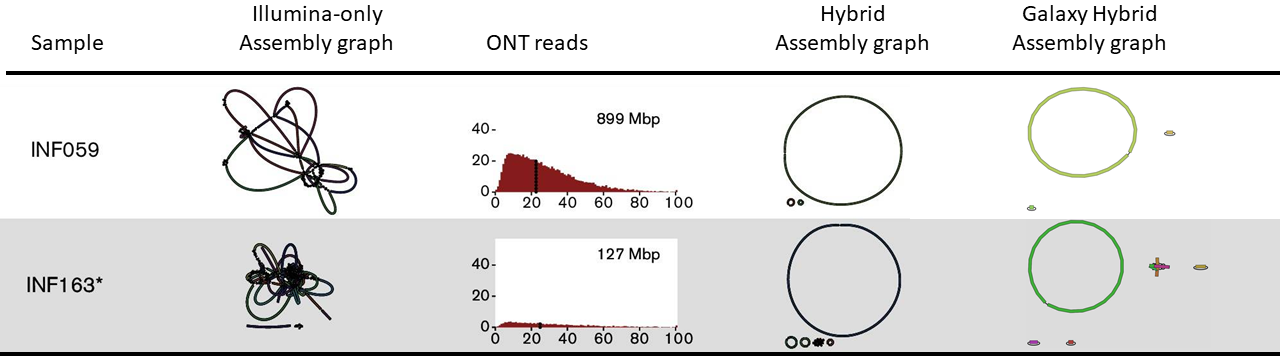
\includegraphics[width=\linewidth]{images/unicycler_result.png}
	\caption{Here the output of \citet{Wick2017} is reproduced. The plasmid assembly graphs output created by Bandage are shown to confirm that the workflow works as expected. The length distribution, total yield and N50 of the Oxford Nanopore Technologies (ONT) reads of each \textit{K. pneumoniae} are shown to show the input data.}\label{figure:WickEtAl}
\end{figure}

The results from both workflows show that they can reproduce the outcomes of the source. For other analysis purposes tools can be used as a single instance or combined into novel workflows. This makes it possible to achieve the information desired by the researcher.

\section{Methods}
\subsection{Implementation}
The implementation of the tools and workflows in Galaxy gives a non-programmer the ability to do extensive research on nanopore sequence data without coding. All tools and their dependencies are installed through the Galaxy platform and are managed by the Conda framework for dependency management. The tools and their dependencies are available from the Bioconda Conda channel \cite{Gruning2018}.

\subsection{Training Materials}
To provide end users with the ability to use NanoGalaxy, an online training manual is developed. This manual demonstrates the use of the tools for long read assembly and provides the end to end workflows. The manuals can be found on the Galaxy training materials website \cite{Batut2018}.  

\subsection{Future Work}
Nanopore sequence analysis is fairly new, therefore there are new developments ongoing. These new created tools or updates of the already incorporated tools need to be kept up-to-date in the Galaxy platform. Furthermore, already incorporated tools can be extended with certain functionalities of the original tools that are now lacking.   

\section{Availability of source code and requirements (optional, if code is present)}

\begin{itemize}
\item Project name:~NanoGalaxy
\item Project home page:~\url{https://nanopore.usegalaxy.eu}
\item Training Manual:~\url{https://galaxyproject.github.io/training-material/topics/metagenomics/tutorials/plasmid-metagenomics-nanopore/tutorial.html}
\item License: GNU GPL
\end{itemize}

\section{Availability of supporting data and materials}

The data presented here to illustrate the functionality of the tools was obtained from previous publications, and has been collected and made available from Zenodo \cite{TODO}.

\section{Declarations}

\subsection{List of abbreviations}

\begin{itemize}
\item AMR: Antimicrobial Resistance
\item NGS: Next Generation Sequencing
\item OECD: Organisation for Economic Co-operation and Development
\item ONT: Oxford Nanopore Technologies
\item SNPs: Single Nucleotide Polymorphisms
\item WHO: World Health Organization
\end{itemize}

\subsection{Competing Interests}
The authors declare that they have no competing interests.

\subsection{Funding}
This project was made possible with the support of ...


\subsection{Author's Contributions}
WK and SH contributed to the tool development and writing of the manuscript.


\section{Acknowledgements}
The authors would like to thank the Galaxy community for their help in reviewing, testing, and validating the tools presented here.

%% Specify your .bib file name here, without the extension
\bibliography{paper-refs}

\end{document}
